%% 
%% Copyright 2007-2020 Elsevier Ltd
%% 
%% This file is part of the 'Elsarticle Bundle'.
%% ---------------------------------------------
%% 
%% It may be distributed under the conditions of the LaTeX Project Public
%% License, either version 1.2 of this license or (at your option) any
%% later version.  The latest version of this license is in
%%    http://www.latex-project.org/lppl.txt
%% and version 1.2 or later is part of all distributions of LaTeX
%% version 1999/12/01 or later.
%% 
%% The list of all files belonging to the 'Elsarticle Bundle' is
%% given in the file `manifest.txt'.
%% 
%% Template article for Elsevier's document class `elsarticle'
%% with harvard style bibliographic references

\documentclass[preprint,12pt,authoryear]{elsarticle}
%\documentclass[10pt,final,journal,compsoc,a4paper]{IEEEtran}
%% Use the option review to obtain double line spacing
%% \documentclass[authoryear,preprint,review,12pt]{elsarticle}

%% Use the options 1p,twocolumn; 3p; 3p,twocolumn; 5p; or 5p,twocolumn
%% for a journal layout:
%% \documentclass[final,1p,times,authoryear]{elsarticle}
%% \documentclass[final,1p,times,twocolumn,authoryear]{elsarticle}
%% \documentclass[final,3p,times,authoryear]{elsarticle}
%% \documentclass[final,3p,times,twocolumn,authoryear]{elsarticle}
%% \documentclass[final,5p,times,authoryear]{elsarticle}
%% \documentclass[final,5p,times,twocolumn,authoryear]{elsarticle}

%% For including figures, graphicx.sty has been loaded in
%% elsarticle.cls. If you prefer to use the old commands
%% please give \usepackage{epsfig}

%% The amssymb package provides various useful mathematical symbols
\usepackage{amssymb}
\usepackage{amsmath}
\usepackage{amsfonts}
\usepackage{pgf-pie}
\usepackage{calc}
\usepackage{graphicx}
\usepackage{float}
\usepackage{anyfontsize}
\usepackage{pgfplots}
\usepackage{amsmath}


%% The amsthm package provides extended theorem environments
%% \usepackage{amsthm}

%% The lineno packages adds line numbers. Start line numbering with
%% \begin{linenumbers}, end it with \end{linenumbers}. Or switch it on
%% for the whole article with \linenumbers.


\addbibresource{references.bib} %Imports bibliography file


\journal{Energy and Buildings}

\begin{document}

\begin{frontmatter}

%% Title, authors and addresses

%% use the tnoteref command within \title for footnotes;
%% use the tnotetext command for theassociated footnote;
%% use the fnref command within \author or \affiliation for footnotes;
%% use the fntext command for theassociated footnote;
%% use the corref command within \author for corresponding author footnotes;
%% use the cortext command for theassociated footnote;
%% use the ead command for the email address,
%% and the form \ead[url] for the home page:
%% \title{Title\tnoteref{label1}}
%% \tnotetext[label1]{}
%% \author{Name\corref{cor1}\fnref{label2}}
%% \ead{email address}
%% \ead[url]{home page}
%% \fntext[label2]{}
%% \cortext[cor1]{}
%% \affiliation{organization={},
%%            addressline={}, 
%%            city={},
%%            postcode={}, 
%%            state={},
%%            country={}}
%% \fntext[label3]{}

\title{Developing sustainable Irish homes in changing TIMES}
%TIMES Ireland Model: Residential Sector
% The changing TIMES of Irish Homes
% Developing sustainable homes in changing TIMES

\author[inst1,inst2]{Jason Mc Guire\footnote{Contact: j.mcguire@ucc.ie}}

\affiliation[inst1]{organization={Energy Policy and Modelling Group, MaREI Centre},%Department and Organization
            addressline={Environmental Research Institute}, 
            city={Cork},
            country={Ireland}}
            
\affiliation[inst2]{organization={School of Engineering},%Department and Organization
            addressline={University College Cork}, 
            city={Cork},
            country={Ireland}}


\author[inst1,inst2]{Fionn Rogan}
\author[inst1,inst2]{Olexandr Balyk}
\author[inst1,inst2]{Hannah Daly}
\author[inst1,inst2]{ \& Brian Ó Gallachóir}

\begin{abstract}
%% Text of abstract
%Ireland's residential sector has particularly underachieved in previous climate targets. Located on the peripherals of Europe, with a high share of low thermal efficient detached dwellings with carbon intensive heating fuels, provides some distinctive barriers to decarbonising Ireland's residential sector. The disadvantageous starting position has impeded residential decarbonisation progress thus far. \par
%Energy system optimization models (ESOMs) have been used extensively to inform pathways in addressing long-term energy challenges which provides insights to decision makers on issues related to climate and energy policy. \par
%The TIMES-Ireland Model (TIM) is a newly developed optimisation model of the Irish energy system, which calculates the  cost-optimal decarbonisation pathway to meet future energy service demands while achieving Ireland's legally binding 2030 and 2050 climate targets.
Write after paper is completed 
 
\end{abstract}

%%Graphical abstract
%%\begin{graphicalabstract}
%%\includegraphics{grabs}
%%\end{graphicalabstract}

%%Research highlights
%%\begin{highlights}
%%\item Research highlight 1
%%\item Research highlight 2
%%\end{highlights}

\begin{keyword}
%% keywords here, in the form: keyword \sep keyword
Energy systems optimisation model (ESOM) \sep The integrated MARKAL-EFOM system (TIMES) \sep Building decarbonisation \sep Model description \sep Residential energy transition
%% PACS codes here, in the form: \PACS code \sep code
%%\PACS 0000 \sep 1111
%% MSC codes here, in the form: \MSC code \sep code
%% or \MSC[2008] code \sep code (2000 is the default)
%% \MSC 0000 \sep 1111
\end{keyword}

\end{frontmatter}

%% \linenumbers

%% main text
\section{Introduction}
\label{sec:Introduction}

Understanding residential energy consumption in Ireland is key to exploring future residential decarbonisation pathways, and interpreting the results. Section \ref{sec:Introduction} looks at Ireland's climate targets, energy policy and distinctive residential sector, before examining how researchers have previously used Energy system optimization models (ESOMs) to analyse the residential sector.
\par Section \ref{LitR} describes the methodology used to develop the residential sector while also describing the input data, along with the applied constraints, technologies, costs and demands.  
Section \ref{Results} outlines the results obtained from selected scenarios. Section \ref{Discussion} discusses the strengths and weakness of the newly developed model and how it differs from other models. Lastly, section \ref{Conclusion} draws some conclusions on the model, results and suggestions on future work which would be beneficially for policy makers in Ireland.

 
\subsection{Ireland: Residential Sector}
\label{Intro:IreRSD}

Ireland’s distinctive energy sectors are further separated from other EU member states when focusing on the residential sector. This is largely down to Ireland’s high reliance on fossil fuels, low building thermal efficiency, larger dwellings and rural settlement patterns. This is illustrated by the fact only 5.8\% of the population of Ireland were living in apartments in 2018, the lowest in EU-27 and well below the 25.3\% average \cite{EurostatDistributionSurveyilc_lvho01}, furthermore 71.4\% of the Irish population are deemed to be living in dwellings too large, where the EU-27 rate is 33\% \cite{EurostatShareSurveyilc_lvho50a}. The low thermal efficiency of Ireland's dwelling stock is highlighted by two facts, firstly the 2021 building regulations require a 70\% reduction of CO2 emissions in new dwellings compared to 2005 \cite{DepartmentofHousingGov.ieBuildings}, and secondly according to Central Statistics Office (CSO) data approx. 85\% of residential buildings are 2005 or older. Furthermore Irelands fossil fuel dependency is underpinned by home heating oil accounting for the largest share of fuel usage in the residential sector at 37\% \cite{SustainableEnergyAuthorityofIreland2018EnergySector}, of which all is imported \cite{OCleirigh2020ENERGYReport}.

In the last 30 years, the extraction of indigenous peat has declined and consequently peat consumption has halved, in 2018 peat accounted for 12.3\% of residential GHG emissions. Residential coal GHG emissions has also declined to 6.9\% in 2018 \cite{Howley2005ENERGY-RELATEDIreland}. However, the decline in peat and coal has been offset by more significant growth in oil in the same period, where oil accounted for 34.8\% of residential GHG emissions in 2018 \cite{Howley2005ENERGY-RELATEDIreland}. Gas availability is limited to some urban areas, and accounted for 15.5\% of residential GHG emission in 2018 \cite{Howley2005ENERGY-RELATEDIreland}. 
The residential sector relied on fossil fuels for over 90\% of thermal energy in 2018, consequently Ireland currently has the lowest renewable heat of among EU member states, at only 6.3\% \cite{Eurostat2021ShareSourcesnrg_ind_ren}. Preliminary results from the Environmental Protection Agency (EPA) have indicated a 9\% increase of residential GHG emissions in 2020, mainly due to low home heating oil prices and covid-related restrictions.

\subsubsection{Current Greenhouse Gas Emissions}
\label{Intro:GHG}

Under 2006  Intergovernmental Panel on Climate Change (IPCC) guidelines, Ireland’s residential sector accounted for 14.2\% of GHGs emissions in 2018 \cite{Howley2005ENERGY-RELATEDIreland}. Focusing on energy-related GHG emissions only, the residential sector directly accounts for 24\% of GHG emissions. Fig. \ref{fig:Ireland2018GHG} shows the energy related GHG disaggregated between transport, heat and electricity. 

\begin{figure}[!htbp]
    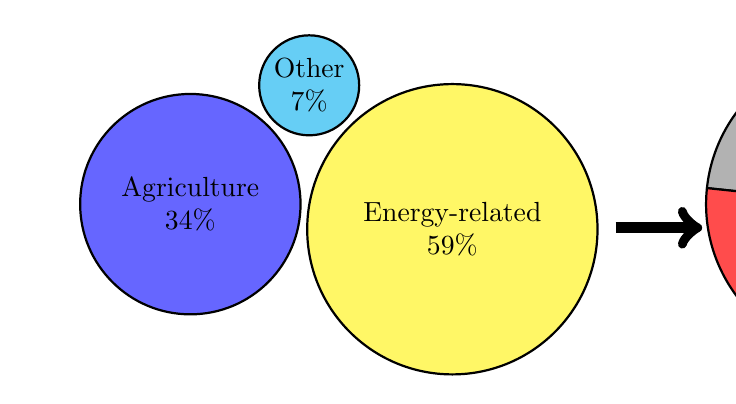
\begin{tikzpicture}[every node/.style={align=center}, pin distance=17mm]
    \pie[cloud,text=inside,radius = 2.4]{34/Agriculture,7/Other,59/Energy-related}
    \draw [->, line width=4pt] (5.4,-0.3) -- (6.5,-.3);
    \hspace{8.5cm}
    \pie[rotate =30,text=inside,radius=1.95,color={black!30,red!70,yellow!40}]{40/Transport,33/Heat,27/Electricity}
    \end{tikzpicture}
    \caption{Ireland 2018 GHG Share \cite{Howley2005ENERGY-RELATEDIreland}}
    \label{fig:Ireland2018GHG}
\end{figure}

Where the residential sector is the direct source 47\% of heat and 30\% of electricity GHG emissions, the residential sector is therefore a pivotal sector in decarbonising energy in Ireland. 



\subsection{Climate Targets}

Under the Climate Action and Low Carbon Development (Amendment) Act 2021, the Irish government has proposed legally binding national targets to reduce Greenhouse Gas (GHG) emissions by 51\% in 2030 compared to 2018. The Act also proposes a long-term target to achieve a climate neutral economy or ``net-zero" by 2050 \cite{2021Climate2021}. These targets accounts for all GHGs - both Emission Trading System (ETS) emissions and non-ETS emissions, and sets out make sectoral five year carbon budgets  a legal requirement to aid progress of the forementioned long-term targets. 
\par The EU's first Nationally Determined Contribution (NDC) which had a 40\% GHG reduction target (first NDC), has been succeeded by a new target of at least a 55\% GHG reduction target (updated NDC) by 2030 compared to 1990 levels \cite{SUBMISSIONSTATES}. Ireland's Climate Action Plan 2019 (CAP2019) complies with EU's first NDC, from which Irelands 30\% Non-ETS GHG reduction target in 2030 compared to 2005 levels was derived  \cite{DepartmentofCommunicationsClimateActionandEnvironment2019Climate2019}. Climate Action Plan 2021 will have to be more ambitious than its predecessor, CAP2019 as it must reflect EU's updated NDC target and take account of the national target also.
There are also renewable energy targets to consider for transport (RES-T), heat (RES-H) and electricity (RES-E) under renewable directive (EU) 2018/2001, and energy efficiency targets under (EU) 2018/2002.

\subsection{Current Energy Policy}
\label{Intro:Policy}
Ireland has set out national policy objectives under 10 strategic investment priorities \cite{Ireland2018ProjectFramework}. The first strategic investment priority is ``Compact Growth" which aims to  achieve \textit{``effective density and consolidation, rather than more sprawl of urban development, [as] a top priority"}. The densification of Ireland's main cities, will provide opportunities to improve the efficiency of heating, electricity and transport within and between cities. 
\par Specifically focusing on the energy sector, the Marginal Abatement Cost Curve (MACC) produced in CAP2019  \cite{EPA2018EPAReport} found electricity \& transport are most cost effective sectors for energy decarbonisation \cite{DepartmentofCommunicationsClimateActionandEnvironment2019DecarbonisationIreland}. CAP2019 findings show the most cost effective solution to decarbonising the residential sector, is to receive higher amounts of low carbon electricity.



%The CAP2019 MACC, shown in Fig.\ref{fig:CAP2019:MACC} provides $>300$ of the most cost-effective technologies options to reduce Non-ETS GHG by 30\% in 2030 compared to 2005 levels. 
%The x-axis (width of each bar chart) shows the potential reduction of annual $MtCO2_{eq}$. The y-axis (height of each bar chart ) shows the associated average cost of abating one tonne of $CO2_{eq}$ over the 2021 to 2030 period. The columns are organised from the most economical (left side) to the most expensive technology (right side) in $EUR/tCO2_{eq}$ \cite{DepartmentofCommunicationsClimateActionandEnvironment2019Climate2019}.
%The options specific to the residential sector are: 

%\begin{itemize}
%    \item{Retrofit oil boiler existing dwellings to B2 equivalent}
 %   \item{Switch from oil boilers to heat pumps in existing dwellings}
 %   \item{Retrofit gas boiler and solid fuel stove existing dwellings to B2 equivalent}
 %   \item{Introduce CO2-free heating in new buildings}\cite{DepartmentofCommunicationsClimateActionandEnvironment2019Climate2019}
%\end{itemize} 

%\begin{figure}[!htbp]
 %\centering
 %\includegraphics[scale=1]{Figures/CAP2019MACC.png} 
 %\caption{Climate Action Plan 2019 - Marginal Abatement Cost Curve}
% \label{fig:CAP2019:MACC} \cite{DepartmentofCommunicationsClimateActionandEnvironment2019Climate2019}
%\end{figure}
%For example, Figure \ref{fig:CAP2019:MACC} shows the retrofitting of oil boilers is expected to reduce the Total Cost of Ownership (TCO) (ie. save money), but only abate a small amount of carbon, whereas switching oil boilers to heat pumps will increase TCO (ie. cost money) but the expected abatement of carbon is far greater. 

In Ireland the decarbonisation of the electricity is underway, with carbon intensity falling annually to 375 $gCO_2/kWh$ in 2018, which is 40\% lower than 2005 levels \cite{Howley2005ENERGY-RELATEDIreland}. 
Ireland uses both the \textit{carrot} (subsidy) and \textit{stick} (tax) approach to direct private invesvestment towards low carbon or renewable energy. A €15/ $tCO_2$ carbon tax was introduced in 2009 to reduce investment in fossil fuels, and the increasing carbon tax rate has resulted in tax receipts growing every year from 2010 to 2018 \cite{Oireachtas2019AnOffice}. Ireland's current carbon tax of €33.50/ $tCO_2$ will rise to €100/ $tCO_2$ in 2030. The Renewable Energy Feed-in Tariff (REFIT) schemes were designed to incentivise renewable electricity investment to achieve legally binding renewable targets under 2009/28/EC. REFIT operates by guaranteeing a minimum price for electricity over a 15 year period. The Renewable Electricity Support Scheme (RESS) replaced REFIT in 2020. RESS supports to renewable electricity projects to help Ireland achieve 2030 climate targets, especially the 70\% renewable electricity target. 
% Almost 800 MW of solar has been approved in RESS-1 \cite{Eirgrid2020RenewableResults}, this greatly exceeds the current solar capacity of 16 MW, while making significant progress towards the CAP2019 target of 1500 MW solar by 2030.
\par Sustainable Energy Authority of Ireland (SEAI) have a key role in the rollout of retrofitting and heat pumps in existing homes. In parallel, new dwellings must achieve a minimum of 20\% renewable energy. The ambient heat used in heat pumps is included as a renewable energy, heat pumps are therefore the preferred heating technology despite the high capital costs. As mentioned in Section \ref{Intro:IreRSD}, new buildings in Ireland produce 70\% less GHG emissions than building in 2005, and with CAP2019 plans to upgrade 500,000 existing homes to a Building Energy Rating (BER) ‘B2’ by 2030, highlights the energy efficiency first approach in the residential sector. 
\par Gas Network Ireland (GNI) have set a 18\% biomethane target for 2030 \cite{Ervia2019VisionIreland}, where CAP2019 only set a 3\% biomethane target for 2030 \cite{DepartmentofCommunicationsClimateActionandEnvironment2019Climate2019}. GNI anticipates that by 2026 or 2027 the supply from Corrib ( Irelands only indigenous gas supply, which provided 61\% of gas in 2018 ) will be less than 30\% of 2018 levels \cite{OCleirigh2020ENERGYReport}. The gas network currently reaches 40\% or 680,000 dwellings in urban areas, but with the ``Compact Growth" policy strategy a higher share of building may have access to the gas network in the future. A major barrier to increasing biomethane from an agricultural source in the gas network is the cost, it was the most expensive option in the Marginal Abatement Cost Curve (MACC) produced in CAP2019.
\par Ireland has one of the lowest shares of District Heating (DH) in Europe at less than 1\%  \cite{Gartland2016AIreland}. The ``Compact Growth" policy strategy and advancement in DH control will strengthen the case for DH networks to play a part in decarbonisaing the residential sector. CAP2019 plans to have approx. 0.4\% of heating provided by DH in 2030, research using TIMES and EnergyPLAN has shown that 37\% of heating provided by DH is optimal if Ireland is to reduce GHG emissions by 80\% in 2050, compared to 1990 \cite{Thellufsen2019ImplementingIreland}. While Irish District Energy Association (IrDEA) suggest 57\% of heat can be sourced from DH, if supporting policy and regulation was in place. District Heating will likely play a role, however Gartland points out a range of organisational, technical, regulatory and economic barriers to DH growth in Ireland \cite{Gartland2016AIreland}. 
\par While it maybe optimal to use Hydrotreated Vegetable Oil (HVO) in transport, it is also considered in the residential sector, as it can provide a cheap alternative for the 700,000 Irish dwellings using home heating oil ( mostly kerosene). HVO which meets the EU sustainability criteria, reduces GHG emissions by 60\% as compared to fossil fuels \cite{Soam2019FactorsSweden}. The capacity of HVO is growing in Europe, but HVO is currently about twice the price of kerosene. HVO can be used to replace kerosene, albeit with cost of up to €400 per oil boiler, however there is no policy for HVO in the residential sector. 

\subsection{Residential Modelling}
\label{Intro:ESOM}

Energy System Optimisation Models (ESOMs) can be used to explore least cost pathways, as they consider a large amount of variables to satisfy demand, while accounting for complex sectoral interconnections within each time period. Some of the main ESOM frameworks include EnergyPLAN \cite{stergaard2015ReviewingSimulations}, MESSAGE \cite{Messner1995WorkingE}, TIMES \cite{Loulou2016DocumentationI}, Balmorel \cite{Wiese2018BalmorelModel}, TEMOA \cite{Hunter2013ModelingTemoa} and OSeMOSYS \cite{Howells2011OSeMOSYS:Development.}.While ESOM cover all the energy-related sectors, they can also be used to specifically explore the residential sector in higher detail, some examples are outlined in this section. 
\par For example, Li et al. \cite{Li2018IncorporatingModel} investigated the heating technology preference in UK, using UK TIMES Model (UKTM). As TIMES \cite{Loulou2016DocumentationI} assumes perfect foresight and \textit{``in reality, the behaviours of consumers is not always economically rational"} \cite{Li2018IncorporatingModel}. Li set out to incorporate a Discrete Choice Model (DCM) into TIMES to better reflect how homeowners choose heating technologies. The DCM was developed from a nationwide survey with 442 homeowners completing the survey. The nationwide survey identified the most influential factors for determining homeowners' preferences for heating systems. The DCM then estimated the probability of a heating technology selection and cost was found not to have a statistically significant impact on homeowners' choices. While Li's researcher has provided some initial insights, future work can improve the robustness and comprehensiveness of the insights, through more surveys and analysis.

Leibowicz et al. developed an expanded version of the Open Source Energy Modeling System (OSeMOSYS) \cite{Howells2011OSeMOSYS:Development.} that integrates electricity generation and storage, residential building energy service demands, and end-use technologies for providing those services \cite{Leibowicz2018OptimalServices}.
Endogenous constraints on the market penetration rate of each technology and hourly service demand profiles are established and applied to the residential sector of Austin, Texas. Austin was chosen because of the high granularity data availability \cite{EnergyInc.}. Leibowicz et al. find, net present costs in the \textit{``Policy scenarios"} ( emissions must decline linearly toward 10\% of their current level by 2050) are higher than \textit{``No Policy scenarios"} (No $CO_2$ regulations will be imposed over the model timeframe), but the percentage increase in net present cost due to the policy diminishes with a more thermally efficient building stock. Leibowicz et al. also finds electrification to be the dominant strategy for cost-effectively decarbonizing urban residential dwellings. 
These insights show the strength of an ESOM, but the not all costs are taken into account in Leibowicz study, the capital cost associated with more thermally efficient buildings are not included.

Hedegard and Münster \cite{Hedegaard2013InfluenceOperation} utilised the ability of Balmorel \cite{Wiese2018BalmorelModel} model to handle the integrated power and district heating system to analyse how heat pumps with  complementing heat storages affect wind power investments in Denmark. The model was disaggreated between a western and eastern Denmark region and the model covers Norway, Sweden, Finland and Germany, in order to cover import/export. Exogenous user constraints applied to the model, based on current Danish policy includes: Wind power must in Denmark by 2020 correspond to at least 50\% of the national electricity consumption, coal is phased out in heat and power plants by 2030, Individual oil boilers are phased out by 2030 and 1.2 Mtonnes straw and 0.2 Mtonnes wood chips must be incinerated at Danish heat and power plants annually. The results by Hedegard and Münster find when investments in individual heat pumps are allowed, air–water heat pumps are installed in non-district heating areas. 
This represents a significant electricity demand in identifying individual heat pumps as highly competitive and can contribute significantly to facilitating larger wind power investments and reducing system costs, fuel consumption, and $CO_2$ emissions.
Hedegard and Münster found the system benefits of adding individual heat storage to the heat pumps are moderate, the main benefit is a reduced need for peak/reserve capacity investments of about 300–600 MW, corresponding to the size of a large power plant. While Balmoral model has provided insights, it does not cover all aspects of the power and heat system, such as start-up costs, minimum load requirements, or part load efficiencies. Nevertheless, the insights are valuable and the results can be soft-linked to other models for deeper analysis. 

Marczinkowski and Østergaard \cite{Marczinkowski2018ResidentialSystems} use EnergyPLAN model \cite{stergaard2015ReviewingSimulations} to explore the feasibility of photovoltaic (PV) systems installed at household level in combination with batteries in Samsø, which is known for being Denmark’s renewable energy island. 
The two approaches are observed for the location of the batteries in the PV system; communal battery system or an individual residential battery approach. The PV/battery combination is but one out of many potential energy technology combinations, but it insights to the optimisation of the energy system in Samsø. 
Marczinkowski and Østergaard found communal batteries slightly more favourable from a technical energy systems perspective, one reason for this is the wind power could also be stored in communal batteries. From the households’ perspective, the first leads to higher, one results showed with identical battery capacity 64\% of electricity demand is satisfied by a residential battery and 36\% by a one communal battery, but the advantage of a energy system model is the integration of other economic sectors in the energy system. While the battery location was explored, the PV system location was not, further investigation into the optimal PV system location could provide further insights. The household occupancy behaviour with and without household batteries on the PV system could alter the optimal pathway.

% NOT INCLUDE HAVE ENOUGH Petrovic and Karlsson \cite{Petrovic2016ResidentialSystem}  examined a new approached to represent residential heat pumps in Denmark 

Many bottom-up models have been used previously to specifically explore Ireland's residential sector \cite{Dineen2011ModellingHeating}\cite{Ahern2013StateStock}\cite{Ahern2015EnergySystems}\cite{Dineen2015ImprovedSource}\cite{Uidhir2020ResidentialIreland}\cite{Uidhir2020ImprovingDecisions} and some models have been used to optimise Ireland's entire energy system \cite{Chiodi2013ModellingSystem}\cite{Connolly2021AalborgEnergy-System}, but very few models have used energy system optimisation model to explore the Irish residential sector. In 2014, Rogan et al used OSeMOYOS to explore energy service demands \cite{Rogan2014LEAPsSystem}, and Thellufsen examining DH with EnergyPLAN and TIMES in 2019 \cite{Thellufsen2019ImplementingIreland}. 

\section{Methodology}
\label{LitR}
% The technical bottom-up development approach of the residential sector is combined with other economic sectors to meet macroeconomic defined demands, to provide GHG targets insights both the energy system and residential sector.

%``How should Ireland set GHG targets in the residential sector?” 
%Choosing the Pathways which Create the Least Burden and Offer the Most Opportunity for Ireland

\subsection{TIMES Energy System Optimisation Model}
\label{Overview}
\par  The expertise among energy policy researchers in Ireland combined with the global network of Energy Technology Systems Analysis Program (ETSAP) modellers, makes TIMES the preferred ESOM to explore Ireland's decarbonisation pathways. Previous versions of the Irish TIMES model were extracted from the Pan European TIMES model, and then updated with specific national data and assumptions. The previous Irish TIMES models were used to provide informative reports on Irish climate policy \cite{Gallachoir2012EPAModel,Deane2017Irish2,Gallachoir2020The3,Deane2013TechnicalIreland,IrishGovernment2017National2017}.  
There is a need for a new ESOM to be built specifically to explore Ireland's new 2030 and 2050 climate targets and sectoral five-year carbon budgets, the new``TIMES Ireland Model" (TIM) was built in 2021 to address this need \textbf{(SOURCE)}.
\par The Integrated MARKAL-EFOM System (TIMES) modelling framework was utilised to develop the Irish model outlined in this paper. TIMES has been developed and maintained by ETSAP of the International Energy Agency (IEA). TIMES is a bottom-up optimisation energy-environment model with perfect foresight which is used to analyse various levels of spatial, temporal and sectoral resolution. Numerous exogenous technical, physical, and regulatory constraints can be are applied to each region and generation technologies have specified fuel types, efficiencies, fixed costs, variable costs, lifetime, capacities, availability factors and environmental characteristics. TIMES uses a linear programming optimizer matrix in General Algebraic Modeling System (GAMS), to compute all calculations. 

\par The function of partial equilibrium operates whereby prices and quantities in each time period are such that the suppliers produce exactly the quantities demanded by the consumers and therefore the total economic surplus  (sum of the suppliers’ and consumers’ surpluses) is maximized \cite{Loulou2016DocumentationI}. The partial equilibrium creates a stable market situation, from which the maximized surplus is first transformed into an equivalent cost minimization objective by taking the negative of the surplus, and calling this value the total system cost. The TIMES objective is therefore to minimize the total `cost' of the system, the TIMES objective function is:
\begin{equation} 
\begin{split}
NPV = {\sum_{r=1}^{R}  \sum_{y\in YEARS}(1 + d_{r,y})^{REFYR-y}}
\cdot {ANNCOST(r,y)} 
\end{split}
%\[ \sum_{n=1}^{\infty} 2^{-n} = 1 \]
\label{Eq:ObjectiveFunction}
\end{equation}
Where: $NPV$ is the net present value of the total cost for all regions ; $ANNCOST(r,y)$ is the total annual cost in region r and year y; $d_{r,y}$ is the general discount rate; $REFYR$ is the reference year for discounting; YEARS is the set of years for which there are costs; and $R$ is the set of regions in the area of study.

With update technological and macroeconomic data, structured specifically to analyse for sectoral five-year carbon budgets towards 2030 and 2050, it is hoped TIM will provide further and more robust insights than previous Irish TIMES model. While also accounting for more fuels and technological options, the residential sector in TIM is structured with around retrofitting, not vice-versa as previous versions, so that it is more aligned to ongoing climate mitigation investments. Also, the residential sector in TIM has also been structured concurrently and similarly to a new Irish LEAP model, to allow more accessible soft-linking. 

%Add description of TIMES and how residential sector is represented to the Methodology section; - Olex Email
%The TIMES-Ireland Model (TIM) is an optimisation model of the Irish energy system, which calculates the cost-5optimal fuel and technology mix to meet future energy service demands in the transport, buildings, industry and agriculture sectors, while respecting constraints in greenhouse-gas emissions, primary energy resources and feasible deployment rates.

%What does new model do that previous didn’t?
%TIM residential improvements - DH, HVO, Solar ( in progress ), better graps the cost and savings of retrofits and heat pumps, which can infrom MACC.Build with 2018 baseyear, not 2010 as previous versions had - this suits the 2030 target
%THe implications of net-zero
%Does new policy context require new modelling approach?
%Yes, do account for ongoing investments in climate mitigation opitions, the approach should provide higher granularity for likely pathways
%How does new modelling structure provide insights (give examples) in a way that previous model didn’t?
%Demands - 
%Improved more detailed Energy Service Demands


\subsection{Residential}
\label{LitR:RES}

%PICKUPHERE
\begin{figure}[!htbp]
 \centering
 \includegraphics[scale=1]{Figures/TIM_Residential_RES (1).jpg}
 \caption{Residential Sector - Reference Energy System}
 \label{fig:RES}
\end{figure}
Behavioral Constraints here 
RES FIGURE 
ENERGY CONSUMPTION CHARACTERISTICS of Houses - 
 %The BER database, which represents half of the dwelling stock, highlights the affect year of construction has on expected energy consumption, as shown in Fig.\ref{fig:BERAge}. The BERs labels are categorised based on expected energy consumption, with A1 representing the lowest expected energy consumption ($\leq 74 kWh/m^2/year$) and G representing the highest expected energy consumption ($ >450 kWh/m^2/year$). The BERs are developed from the Energy Performance of Buildings Directive 2002/91/ EC, which helps to better understand the housing stock. BERs are required for new houses, rented houses, sold houses and renovated houses. 

\begin{figure}[!htbp]
 \centering
 \includegraphics[scale=0.5]{Figures/BERAge.png}
 \caption{Building Energy Rating by Age}
 \label{fig:BERAge}
\end{figure}

Theoretically G-rated BERs consume more energy and consequently have higher energy bills to maintain a comfortable internal temperature, but in reality G-rated dwellings have low internal temperatures, which is a reason for Ireland's high excessive winter mortality \cite{Clinch2000HousingMortality}. Fuel Poverty which which is defined as when a \textit{``household spends 10\% or more of income to achieve adequate warmth"} is a major contributor to the high excessive winter deaths. An Element Energy report claimed 28\% of Irish households were in fuel poverty in 2015  \cite{ElementEnergy2015Bottom-upIreland}. Fuel Allowance and the Household Benefits provides support to low income households to alleviate fuel poverty. These payments have been increased over time with a further increase made in Budget 2020, coinciding with the increase in the carbon tax \cite{,EuropeanUnion2020EUObservatory}. Kerr's study finds an explicit link between fuel poverty and social welfare policy in Ireland \cite{,EuropeanUnion2020EUObservatory,Kerr2019PoliticsFrance} and O’Meara highlights the health issues associated with Fuel Poverty \cite{OMeara2016AIreland}. Ironically, it can be argued this places low income households deeply dependent on fossil fuels for health.
\par BERs do not take account of actual usage based on occupancy behaviour or occupancy density, nor does it take account of the size of the dwelling. The BER labels do therefore leave a gap between actual consumption and expected consumption, the literature review explains how this problem was tackled.
\subsubsection{House Stock Data}
BER Database, CSO and Calculations and Filtration 
FIGURE - Expected and Actual Consumption per m2
Than Actual 

\subsubsection{Costs}
\label{LitR:Costs}
Elephant in the room - Fuel Poverty
%JF -The tax / subsidy inclusive prices are important in driving behaviour, and taxes and subsidies will be a vital policy instrument. Thus, uptake of technologies such as retrofitting will be driven, inter alia, by the net price for consumers.
\subsubsection{Savings}
\label{LitR:Savings}
\subsubsection{Energy Service Demands Projections}
\label{LitR:Demands}
Macroeconomic 
Time slices - 40 etc. 
% textit{To accommodate an expanding population, the number of dwellings has also increased to currently stand at 1.7 million households, although this fgure remains signifcantly short of projected housing need, withannual average demand estimated to be up to 36,000 units for the next 30 years (IBEC 2018). Yet despite the number of new homes built to ever increasing energy performance standards, the Irish housing stock is among the poorest in Europe in terms of energy effciency (Goggins et al. 2016). Current trends also show that households are getting bigger, with an average 15\% increase in foor area across all homes between 2000 and 2016 (SEAI 2018) \cite{FahyEnergyPractice}}
Check main TIM paper 
Historical population estimates and future projections are obtained from the Central Statistics Office (CSO), Ireland \citep{CentralStatisticsOffice2020}. We use the M2F1 scenario since it represents medium growth in population and is in line with population projections used in other national sources \citep{Yakut2020}. 

\begin{table}[htbp]
\footnotesize
 \centering
 \caption{Energy service demands in TIM}
 
 \begin{tabular}{p{18em}lccc}
 \hline
    \multirow{Energy Service Demand} & \multirow{Driver} & \multicolumn{2}{c}{Value} & \multirow{Unit} \\
          &       & \multicolumn{1}{c}{2018} & \multicolumn{1}{c}{2050} &  \\ \hline
    Residential Apartment Demand & Population & 206.80 & 628.93 & 000' \\
    Residential Attached Demand & Population & 766.35 & 1056.50 & 000' \\
    Residential Detached Demand & Population & 724.43 & 889.76 & 000' \\
    \hline
    \end{tabular}%

  \label{tab:ESD_list}%
\end{table}%

% Table generated by Excel2LaTeX from sheet 'Population'
\begin{table}[htbp]
 \centering
 \footnotesize
 \caption{Population}
 \begin{tabular}{cc}
 \hline
 Year & Population (millions) \\
 \hline
 2018 & 4.85 \\
 2020 & 4.98 \\
 2030 & 5.40 \\
 2040 & 5.82 \\
 2050 & 6.19 \\
 \hline
 \end{tabular}%
 \label{tab:pop}%
\end{table}%


The residential stock projections upto 2040 are taken from ESRI's housing demand estimates \citep{Bergin2020}. The stock is expected to increase by 40\% from 2018 level with a CAGR of 2\%. This results in an average of 27,600 new houses per annum between between 2021-2040. Beyond 2040, population is used as a driver to project housing stock. The total housing stock obtained in 2050 is 2.57 million which implies 8\% increase from 2040. 
% Table generated by Excel2LaTeX from sheet 'Sheet1'
\begin{table}[htbp]
  \centering
  \footnotesize
  \caption{Number of dwellings by type ('000)}
    \begin{tabular}{rrrr}
    \hline
    \multicolumn{1}{l}{Year} & \multicolumn{1}{l}{Apartment} & \multicolumn{1}{l}{Attached } & \multicolumn{1}{l}{Detached} \\ \hline
    2018  & 207   & 766   & 724 \\
    2030  & 355   & 918   & 833 \\
    2040  & 493   & 1003  & 878 \\
    2050  & 629   & 1057  & 890 \\ \hline
    \end{tabular}%
  \label{tab:addlabel}%
\end{table}%

Space heating is the largest residential energy service demand, accounted for 61.8\% of final energy usage in 2018. Other residential energy services and their share of final energy is shown in Fig.\ref{fig:Ireland2018ServiceDemands}. As building thermal efficiency and heating technology efficiency improves, both space and water heating energy would be expected to decline. The new A-rated dwellings can be used as a guide to show the share of future energy service demands. From the BER database, it can be seen that A-rated dwellings use less than half space heating energy of the average dwelling and A-rated water heating energy decreases by about 40\% compared to the average A-rated dwelling. However Pumps \& Fans energy increases as mechanical ventilation is used over natural ventilation and Lighting usage in A-rated is more than double the average household. Cooking and Appliances energy usage would be expected to remain stable. 


\begin{figure}[!htbp]
\centering
    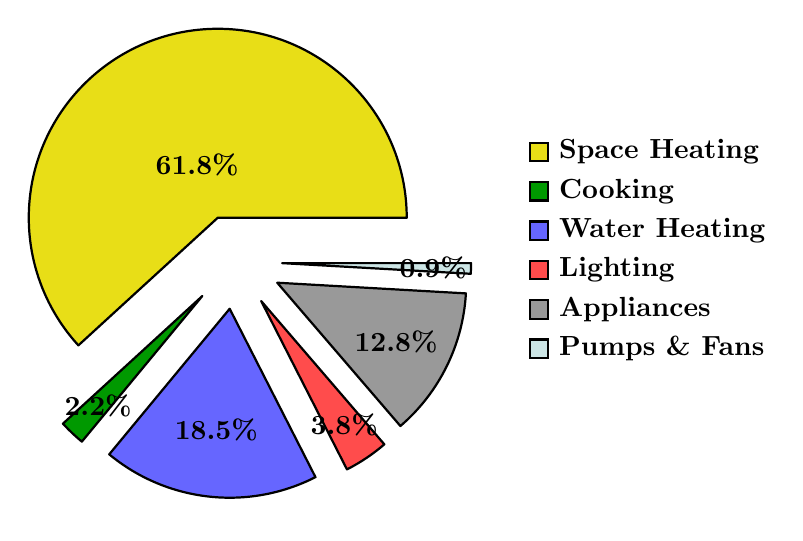
\begin{tikzpicture}
    \tikzstyle{every node}=[font={\bf}]
    \pie[   color = { yellow!90!black, green!60!black, blue!60,
        red!70,
        gray!80,
        teal!20
    }, explode = 0.6, text=legend, radius=2.4]{61.8/Space Heating, 2.2/Cooking, 18.5/Water Heating, 3.8/Lighting, 12.8/Appliances,0.9/Pumps \& Fans}
    \end{tikzpicture}
    \caption{Ireland 2018 Energy Service Demands}
    \label{fig:Ireland2018ServiceDemands}
\end{figure}

Notably absent from Fig.\ref{fig:Ireland2018ServiceDemands}, is space cooling, which is accounted for in appliances. The Policy Oriented Tool for Energy and Climate Change Impact Assessment (POTEnCIA) project disaggregated Ireland's residential space cooling from appliances and have output expected space cooling energy consumption projections are shown in Fig.\ref{fig:Cooling}. 


\begin{figure}[!htbp]
\centering
\begin{tikzpicture}
\begin{axis}[
    x tick label style={
		/pgf/number format/1000 sep=}, xlabel={Year},
	y tick label style={
	    /pgf/number},
		ylabel={Energy Consumption($ktoe$)},
		 scaled y ticks = false,
    xmin=2000, xmax=2050,
    ymin=0, ymax=40,
    xtick={2000,2010,2020,2030,2040,2050},
    ytick={0,10,20,30,40},
    ymajorgrids=true,
]
\addplot[
    color=blue,
    mark=square,
    ]
    coordinates {
    (2000,0.6)(2010,3.1)(2020,8.4)(2030,16.3)(2040,26.1)(2050,37)
    };
    
\end{axis}
\end{tikzpicture}
    \caption{Space Cooling Residential Energy Consumption (Source: POTEnCIA) }
    \label{fig:Cooling}
\end{figure}

The SEAI residential energy report \cite{SustainableEnergyAuthorityofIreland2018EnergySector} provides high resolution detail on energy demands in the residential sector. Variables such as disposable income, appliance ownership, dwelling location, type of occupier status (owner/rented ), BER labels and age of dwelling. 



%Space Heating demand - BER space heating is only within certain months and assumes 21C heating..
Thermostats are not widely used for temperature regulation in private dwellings in Ireland; instead the domestic heating schedule was assumed to be 07.00–09.00 h and 17.00–23.00 h for a heating season of October to May inclusive, based on guidelines issued by the Sustainable Energy Authority of Ireland (SEAI) [32]. The thermal load consists of both space heating and a baseline demand for sustaining water heating. For non-domestic premises the thermal load is defined by office hours, in line with the electrical demand. The domestic thermal loads considered in this study are listed in Table 2; the thermal load for the non-domestic
\subsubsection{Space and Water Heating}
ISO EN 13790 (Energy Performance of Buildings Directive).
Capacity, Efficiency, Constraints, Uptake, adapation
heat output (Qt) and electricity input in a given time per-iod (Pt) is expressed asQt= COPPt, where COP is the average an-nual coefficient of performance for the heat pump
\subsubsection{Lighting, Appliances and Other}
Capacity, Efficiency, Constraints, Uptake, adapation
\subsubsection{User Constraints}
\label{LitR:Constraints}
LIST OF SCENARIOS?
GROWTH CONSTRAINT -A specific type of constraint may be defined to limit the share of process (p) in the total production of commodity (c). The constraint indicates that the flow of commodity (c) from/to process (p) - CommodiTypically, a growth constraint is of the following generic form (ignoring several indices for clarity: \cite{Loulou2016EnergyProgramme}
\begin{equation} 
\begin{split}
VAR\_CAP(t + 1) \leq (1 + GROWTH^{M(t+1)-M(t)}) \cdot VAR\_CAP(t)+K
\end{split}
\label{Eq:GrowthConstraint}
\end{equation}
The GROWTH coefficient is defined as a new attribute of the technology, and represents the maximum annual growth allowed for the capacity. The quantity M(t+1)-M(t) is the number of years between the milestones of periods t and t+1. The constant K is useful whenever the technology has no capacity initially, in order to allow capacity to build over time (if K were absent and initial capacity is zero, the technology would never acquire any capacity)
Note that the sign of the constraint may also be of the "larger than or equal to" type to express a maximum rate of abandonment, in which case the "+" sign is replaced by a "–" sign in the right-hand-side of the constraint. Equality is also allowed, but must be used only exceptionally in order to avoid railroading of the model.
5.4.11

 % LIT REW INPUT DATA - EU \cite{Simoes2013TheProject} 
- LI,er.alThe nationwide survey identified existing technologies, age,
income, region, dwelling characteristics, and knowledge of eco- technology as the six most influential factors for determining homeowners' preferences for heating systems. Among
%the new A-rated houses behave distinctively different which much less demand on space heating and with pumps and fans energy consumption usage increasing, while appliance end use is increasing across the BER ratings. The number of appliances has increased rapidly and while energy efficient improves are  reducing the energy per appliance, it is overshadowed by the growth in electrical appliances. There retrofitting grant which  requires building to have a HLI indication of 2 or less before a heat pump grant can be installs. Ireland’s aim of retrofitting 0.5 million homes from the existing 1.7 million in the before 2030. The effect of these targets also stretches out across the construction sector. The savings from retrofits will decrease fossil fuel energy usage, while most houses 00\% would need to get heat pumps too, to fulfil 0.4 million existing houses getting heat pumps.  This energy efficiency first approach would allow for future technology choices, when current boiler are not at end of life. 

TIM was built to help Ireland provide a pathway to achieve 2030 and 2050 targets. The residential sector plays a key part of this and it was built from the SEAI 2018 energy balance, the BER database and CSO data. The data filtration process used in the residential sector, derived a lot of conversation of the BER database, a group know as Ireland Energy Wiki by the National Retrofitting Modelling Group grew from building the residential sector, questions about the filters, default values, assumptions around thermal equations (EC..) and uncertainties were used to improve the data before it was used in TIM . TIM has many internal project deadines, which required extensive meetings about the data, constraints and results as the modelling was progressing. The data and results were presented to 30 external reviewers to provide feedback, this process proved invaluable having different expertise with different presepectives enabled TIM to fill in gaps. TIM will also be open platform to help improve the model and provide transparency. TIM’s residential sector was built in parallel with LEAP’s residential sector, so that residential sector can easily simulate policy. The demand for results from TIM has increased significantly with increased government ambition, TIM will provide input into CAP 2021 and Ireland’s carbon budgets, working with DECC and the CCAC respectively will also provide feedback and improve the robustness of TIM. for these reasons TIM residential sector is a state of the art modelling platform. 


\section{Results}

\label{Results}
Electricity Supply, Technology and Fuel Mix, Retrofitting, Cost

%% The Appendices part is started with the command \appendix;
%% appendix sections are then done as normal sections
\section{Discussion}
\label{Discussion}
Soft-linking to LEAP and PLEXOS
%o	Discuss and interpret the results
%o	Focus on what added value the model brings
%o	Also include future development priorities here
%o	What can’t the model do? Where is it more suitable to use another model - Hannah Email

\subsection{Strengths}
\label{Dis:Strengths}
\subsection{Limitations}
\label{Dis:Limit}
Consumers’ final investment decision can be
represented by “willingness-to-pay” curves – for
instance, around 10\% of owner-occupiers are willing
to invest in energy efficiency measures for a payback
time of 4 years, falling to 0\% for a payback time of
6 years for some consumer cohorts
\section{Conclusions}
\label{Conclusion}
This paper reports results on ambitious mitigation target in the period to 2050 for the Irish energy system. The analysis have been performed using the Irish TIMES model
\textit{We stress the importance of differentiating between technical con-
straints and behavioural constraints in optimisation models. Including both conflates what is considered desirable under the economic welfare paradigm (i.e. cost-minimising decisions) with “realistic decisions”, complicating the interpretation of the results. Optimisation models are by design well suited to study cost-optimal behaviour, and running scenarios just with technical constraints facilitates the identification of areas where market barriers are more entrenched, and interventions to accelerate the uptake of low-carbon practices may be needed.} \cite{Astudillo2017CanModelb}
\section{Acknowledgements}
\label{sec:Acknowledgements}
Tomas %CAPACITY is funded under the Climate Action Modelling Group (CAMG) by DECC
% https://www.marei.ie/project/capacity/
CHIMERA is supported by a research grant from Science Foundation Ireland (SFI) and the National Natural Science Foundation of China (NSFC) under the SFI-NSFC Partnership Programme, grant no. 17/NSFC/5181 and
supported by MaREI, the SFI Research Centre for Energy, Climate, and Marine [Grant No: 12/RC/2302\_P2]


https://www.marei.ie/project/chimera/
\appendix

\section{Sample Appendix Section}
\label{sec:sample:appendix}
XXXXXXXX

%% If you have bibdatabase file and want bibtex to generate the
%% bibitems, please use
%%

\printbibliography

%% else use the following coding to input the bibitems directly in the
%% TeX file.

%%\begin{thebibliography}{00}


% %% \bibitem[Author(year)]{label}
% %% Text of bibliographic item

% \bibitem[ ()]{}

% \end{thebibliography}
\end{document}
\endinput
%%
%% End of file `elsarticle-template-harv.tex'.
